\subsection{RAG Architecture Overview}
\label{subsec:rag-architecture}

Retrieval-Augmented Generation (RAG) is a hybrid architecture that combines dense document retrieval with generative language models to produce grounded and context-aware answers, as illustrated in Figure 3, which shows the complete pipeline from user query to final response.


\subsubsection*{Core Components}
\begin{itemize}
    \item \textbf{Retriever:} Retrieves relevant documents from a knowledge base using semantic similarity.
    \item \textbf{Generator:} Generates the final answer using the user's query and the retrieved context.
\end{itemize}

\subsubsection*{Workflow}
\begin{enumerate}
    \item \textbf{Query Encoding:}
    The user's question is first embedded into a dense vector using the \texttt{Bge-m3} embedding model, which captures the semantic meaning of the input.
    
    \item \textbf{Document Retrieval:}
    The query vector is used to search the \texttt{ChromaDB} vector store, where document chunks have also been embedded and indexed. The system retrieves the top-$k$ most relevant chunks based on cosine similarity.
    
    \item \textbf{Context Injection:}
    The retrieved chunks are concatenated and formatted as part of the prompt. This contextual information is added before the query to give the language model background knowledge it can reference during generation.
    
    \item \textbf{Response Generation:}
    The prompt, consisting of both the retrieved content and the original query, is passed to the LLM (\texttt{Llama3-2B-Instruct}), which generates a coherent and grounded response. The generated answer is influenced by the evidence provided, increasing factual accuracy.
\end{enumerate}

\subsubsection*{Advantages}
\begin{itemize}
    \item \textbf{Improved Factual Accuracy:} Since answers are based on up-to-date, verified documents, the model is less likely to hallucinate or fabricate information.
    
    \item \textbf{Dynamic Knowledge Updates:} New content can be added to the vector store without needing to retrain the model, allowing continuous updates and scalability.
    
    \item \textbf{Transparent Reasoning:} Retrieved chunks can be shown alongside responses, allowing users (including patients and doctors) to trace the origin of the information and validate it.
    
    \item \textbf{Domain Adaptability:} RAG can be easily tailored to specific domains like medical information, making it highly suitable for our use case involving respiratory health.
\end{itemize}

\begin{figure}[htbp]
  \centering
  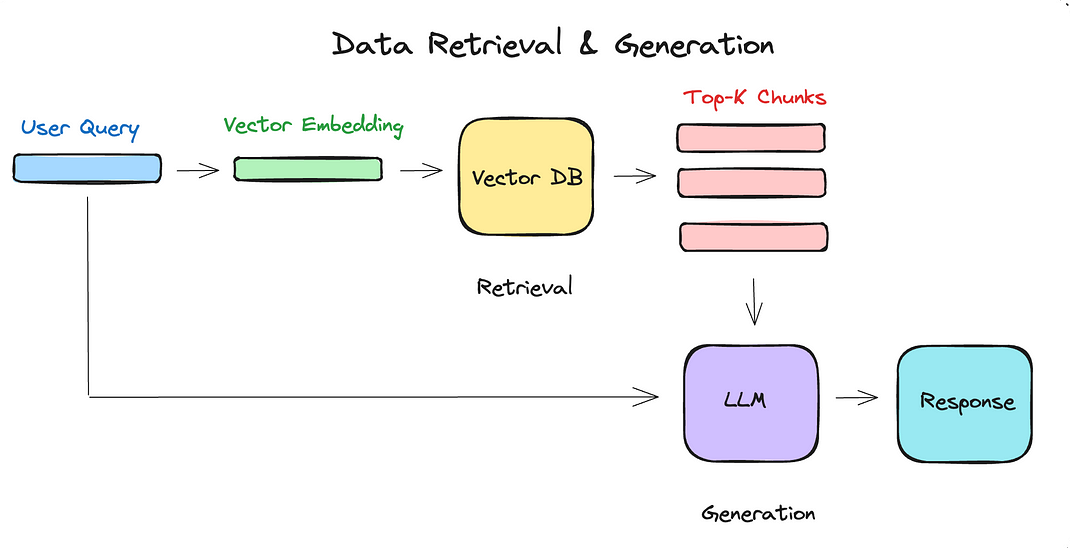
\includegraphics[width=0.8\textwidth]{rapport_pfa-main/images/Data_retrieval_and_generation_RAG.png}
  \caption*{\textbf{Figure 3:} RAG Pipeline} % Starred version
  \label{fig:indexing-process-manual}
\end{figure}

\subsection{Retriever Component}
\label{subsec:retriever}

The retriever is a critical part of the RAG pipeline responsible for identifying and returning the most semantically relevant document chunks in response to user queries.

We implemented a \textbf{dense retriever}, which relies on representing both queries and documents as dense vectors in a shared embedding space. Unlike traditional sparse retrieval methods (e.g., TF-IDF or BM25) that depend on exact keyword matching, dense retrieval captures semantic similarity by measuring the distance between vector representations. This allows retrieval of relevant information even when the exact query terms are not present in the documents.

\subsubsection*{Dense Retriever Mechanism}
Both the query $q$ and each document chunk $d_i$ are embedded into dense vectors:

\begin{equation*}
\mathbf{v}_q = \text{Embed}(q), \quad \mathbf{v}_{d_i} = \text{Embed}(d_i)
\end{equation*}

where $\text{Embed}(\cdot)$ is the embedding function implemented by the \texttt{BGE-M3} model.

The similarity score between the query and each document chunk is computed using cosine similarity:

\begin{equation*}
\text{sim}(\mathbf{v}_q, \mathbf{v}_{d_i}) = \frac{\mathbf{v}_q \cdot \mathbf{v}_{d_i}}{\|\mathbf{v}_q\| \|\mathbf{v}_{d_i}\|}
\end{equation*}

The retriever then ranks all candidate documents based on their similarity scores and selects the top-$k$ documents with the highest scores.

\subsubsection*{Embedding Model: BGE-M3}
To generate these embeddings, we used the \texttt{BGE-M3} embedding model developed by BAAI. This model was selected due to its strong capabilities:

\begin{itemize}
    \item \textbf{Multi-Functionality:} Supports dense retrieval, sparse retrieval, and multi-vector retrieval, making it versatile for different search scenarios.
    
    \item \textbf{Multi-Linguality:} Trained on over 100 languages, enabling support for diverse user inputs.
    
    \item \textbf{Multi-Granularity:} Handles inputs ranging from short queries to long documents (up to 8192 tokens), which suits embedding medical literature and user queries effectively.
\end{itemize}

These characteristics allow \texttt{BGE-M3} to generate rich, meaningful embeddings that improve retrieval quality.

\subsubsection*{Top-K Selection}
The retriever selects the top 3 most relevant document chunks for each query based on cosine similarity between embeddings. This choice was made after analyzing the collected queries and frequently asked questions (FAQ). We found that no more than three documents were generally necessary to provide sufficient context for answering user queries accurately. Setting top-k = 3 balances providing enough relevant information while avoiding excessive or noisy context that could confuse the language model.
This approach ensures the generator receives focused and contextually relevant information, improving the overall response quality.

\subsection{Generator Component}
\label{subsec:generator}

\subsubsection{Language Model Description}
\label{sssec:lm-description}

We used in the generator component the Llama 3.2 1B Instruct model with Q6-K quantization. This model contains approximately 1 billion parameters, offering a balance between computational efficiency and language understanding capabilities. It is specifically fine-tuned on instruction-following datasets, which enables it to interpret and respond effectively to user queries with clear, context-aware, and relevant answers.
The model benefits from Q6-K quantization, a technique that reduces the precision of model weights to 6 bits, allowing for significant reductions in memory usage and faster inference times without substantially sacrificing performance. This makes the model well-suited for deployment in resource-constrained environments, such as mobile applications.
The Llama 3.2 1b Instruct model’s combination of compact size, instruction fine-tuning, and efficient quantization makes it ideal for our AI assistant, enabling fast and reliable generation of medically accurate responses in real-time.


\subsubsection{Instruct-Tuning}
\label{sssec:instruct-tuning}

\paragraph{Objective:} 
 The fine-tuning process aimed to adapt the Llama 3.2 model for instruction-following tasks, enhancing its ability to generate accurate and context-aware responses based on user queries.

\paragraph{Fine-Tuning Methodology:}
Meta employed a combination of Supervised Fine-Tuning (SFT) and Reinforcement Learning with Human Feedback (RLHF) to align the model's outputs with human preferences for helpfulness and safety.

\begin{itemize}
    \item \textbf{Supervised Fine-Tuning (SFT):}
    In this phase, the model was trained on a dataset comprising instruction-response pairs. This supervised approach helped the model learn to follow instructions and generate appropriate responses.
    
    \item \textbf{Reinforcement Learning with Human Feedback (RLHF):}
    Following SFT, RLHF was utilized to further refine the model's behavior. Human feedback was incorporated to guide the model towards producing outputs that align with desired characteristics, such as factual accuracy and helpfulness.
\end{itemize}

\paragraph{Training Data:}
The fine-tuning process utilized a diverse mix of publicly available online data, encompassing various languages and domains. This multilingual dataset enabled the model to perform effectively across different languages and tasks .

\paragraph{Outcome:}
The fine-tuned Llama 3.2 Instruct models demonstrated improved performance on common industry benchmarks, outperforming many existing open-source and closed chat models in tasks requiring instruction-following capabilities .

\subsubsection{Quantization}
\label{sssec: quantization}

Quantization is a widely used technique in deep learning to reduce the computational and memory costs of neural networks by representing weights and activations with lower precision numerical formats. Instead of using 32-bit floating-point numbers (FP32), quantization typically converts these values to 16-bit (FP16), 8-bit, or even lower-bit integer representations such as 6-bit or 4-bit integers.
In our project, we employed \texttt{Q6\_K} quantization, which specifically compresses model weights to 6-bit precision, allowing a significant reduction in model size and inference latency while maintaining strong performance.

\paragraph{Techniques in Quantization:}
There are several methods for quantization, including:

\begin{itemize}
    \item \textbf{Post-Training Quantization (PTQ):} This technique applies quantization after the model has been fully trained. It is fast and does not require retraining but can sometimes lead to accuracy degradation if not carefully tuned.
    
    \item \textbf{Quantization-Aware Training (QAT):} In this method, the model is trained or fine-tuned with quantization in mind. The training simulates quantized weights and activations, helping the model adapt to the lower precision and thus preserving accuracy better.
\end{itemize}

Our use of \texttt{Q6\_K} falls into post-training quantization optimized for language models, focusing on balancing compression and accuracy without retraining the entire model.

\paragraph{How Quantization Works:}
The core idea is to map floating-point weights $w \in \mathbb{R}$ to discrete quantized values $q \in \mathbb{Z}$ using a scale $s$ and zero-point $z$, typically by:

\begin{equation*}
q = \text{round}\left(\frac{w}{s}\right) + z
\end{equation*}

where $s$ scales the real values into the quantization range and $z$ shifts the zero point. In 6-bit quantization, the values are mapped to integers in the range $[0, 63]$.

For inference, the quantized weights are dequantized back to floating-point by:

\begin{equation*}
\hat{w} = s \times (q - z)
\end{equation*}

The challenge is to choose $s$ and $z$ such that the quantized weights closely approximate the original weights and minimize error propagation through the network.

\paragraph{Benefits of Q6\_K Quantization:}
\begin{itemize}
    \item \textbf{Memory Reduction:} Reducing the weight precision from 32-bit to 6-bit reduces model size by over 5 times.
    
    \item \textbf{Inference Speedup:} Integer arithmetic operations on 6-bit numbers are faster and more energy-efficient on compatible hardware.
    
    \item \textbf{Compatibility:} \texttt{Q6\_K} quantization is designed specifically for transformer architectures, preserving their performance better than naïve quantization approaches.
    
    \item \textbf{Minimal Accuracy Loss:} Carefully calibrated quantization parameters help maintain the semantic understanding and generation quality of the language model.
\end{itemize}

\paragraph{Challenges}
\begin{itemize}
    \item \textbf{Quantization Error:} Low-bit precision introduces quantization noise which can degrade model output if not carefully managed.
    
    \item \textbf{Hardware Support:} Efficient execution of 6-bit operations requires specialized hardware or optimized libraries, which might not be universally available.
    
    \item \textbf{Calibration:} Choosing appropriate scale and zero-point parameters requires calibration on representative data to minimize performance loss.
\end{itemize}

Overall, \texttt{Q6\_K} quantization provides an effective trade-off between resource efficiency and model performance, making it highly suitable for deploying \texttt{Llama 3.2 1B Instruct} in our AI assistant, ensuring fast, reliable, and resource-conscious inference.

\subsubsection{Prompt Engineering}
\label{sssec:prompt-engineering}

Prompt engineering is the process of designing and structuring the input provided to a language model to effectively guide its behavior and output. It plays a critical role in ensuring the model understands the task objective, responds appropriately, and uses the provided context efficiently.

In our RAG-based assistant, prompt engineering was essential to help the language model generate relevant, fact-based, and context-aware answers.

\paragraph{System Prompt Design}
We defined a system prompt to instruct the model on its role and expected tone. This was used to prime the model at the beginning of each interaction.

\begin{verbatim}
You are a knowledgeable and compassionate medical assistant chatbot 
specialized in respiratory diseases. Your goal is to help users understand 
symptoms, conditions, prevention, and treatments related to the respiratory 
system. Always provide clear, concise, and medically accurate information 
based on trusted sources. Avoid repetition, stay focused on the specific 
question, and include practical advice when relevant.
\end{verbatim}

This guided the model to behave as a reliable assistant, aligned with the medical nature of the application.

\paragraph{Contextual Prompt Construction} 
When a user submits a query, the top-3 most relevant chunks from the knowledge base are retrieved and injected into the prompt following this structure:

\begin{verbatim}
Question: [User's original question]
Context:
1. [First retrieved knowledge chunk]
2. [Second retrieved knowledge chunk] 
3. [Third retrieved knowledge chunk]

Instruction: Use only the provided context to answer. 
If information is incomplete, respond: "Based on my medical resources, 
I would suggest consulting a healthcare professional about this."
Never speculate beyond the given context.
\end{verbatim}

The prompt explicitly instructs the LLM to: (1) treat the context as primary source but verify completeness, (2) acknowledge limitations when context is insufficient by recommending professional consultation, and (3) strictly avoid fabrication. This design ensures trustworthy responses while minimizing hallucinations and maintaining clinical responsibility - particularly crucial for respiratory health queries where accuracy impacts patient outcomes.

This design ensures that responses are fact-grounded, transparent, and aligned with medical best practices.